\documentclass[letterpaper]{article}
\usepackage[utf8]{inputenc}
\usepackage[spanish]{babel}
\usepackage{amssymb, amsmath}
\usepackage{stackengine}
\usepackage{graphicx}
\usepackage{ mathrsfs }
\usepackage{lipsum}
\usepackage{dsfont}
\usepackage[margin=1.5cm,
vmargin={1.5cm,0.7cm},
includefoot]{geometry}
\usepackage{setspace}
\usepackage{subcaption}
\usepackage{tocloft}
\usepackage{upgreek}
\usepackage{amsthm}
\usepackage{graphicx}
\usepackage{paralist}
\usepackage{fancyhdr}
\usepackage{lmodern}
\usepackage{tcolorbox}
\usepackage{color}
\usepackage{tikz}
\usepackage{wasysym}
\usepackage{textgreek, marvosym}
\tcbuselibrary{skins,breakable}
\pagestyle{fancy}

\renewcommand{\headrulewidth}{0.4pt}
\renewcommand{\footrulewidth}{0.4pt}

\renewcommand{\d}{\partial}

\providecommand{\abs}[1]{\left|#1\right|}
\providecommand{\norm}[1]{\left|\left|#1\right|\right|}														  
\providecommand{\pint}[1]{\langle#1\rangle}														  
\newcommand{\V}{\mathds{V}}

\newcommand{\W}{\mathds{W}}

\newcommand{\F}{\mathds{F}}

\newcommand{\tq}{ \quad \cdot  \backepsilon \cdot \quad }

\newcommand{\ld}{\lim\limits_{x \to 0^{+}}}

\newcommand{\li}{\lim\limits_{x \to 0^{-}}}

\newcommand{\la}{\lim\limits_{x \to a}}

\renewcommand{\l}{\ell}

\newcommand{\R}{\mathds{R}}

\newcommand{\Po}{\mathds{P}_2(\mathds{R})}

\renewcommand{\*}{\cdot}

\newcommand{\Iden}{\begin{pmatrix}
		1 & 0 & 0\\
		0 & 1 & 0\\
		0 & 0 & 1 
\end{pmatrix}}
\newcommand{\T}{\begin{pmatrix}
		1 & 3 & 9 \\
		1 & 3 & 4 \\
		0 & 0 & 2 
\end{pmatrix} }

\makeatletter
\renewcommand*\env@matrix[1][\arraystretch]{%
	\edef\arraystretch{#1}%
	\hskip -\arraycolsep
	\let\@ifnextchar\new@ifnextchar
	\array{*\c@MaxMatrixCols c}}
\makeatother

\newtheorem{theorem}{Teorema}[]
\theoremstyle{definition}
\newtheorem{definition}{Definición}
\newtheorem{lema}{Lema}


\begin{document}
		\setlength{\unitlength}{1cm}
	\thispagestyle{empty}
	\begin{picture}(19,3)
	\put(-0.5,1.2){
\includegraphics[scale=.20]{img/unam1.png}}
	\put(16,1){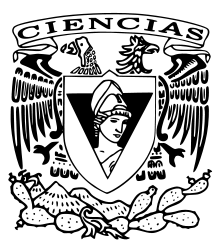
\includegraphics[scale=.29]{img/fciencias1.png}}
	\end{picture}
	
	\begin{center}
		\vspace{-114pt}
		\textbf{\large Matemáticas para las Ciencias II}\\
		\textbf{ Semestre 2020-2}\\
		Prof. Pedro Porras Flores\\
		Ayud. Irving Hernández Rosas \\
		\textbf{Tarea Examen}\\[0.2cm]
		Kevin Ariel Merino Peña\footnote{Número de cuenta 317031326}\\ [0.2cm]
	\end{center}
	\vspace{-10pt}
	\rule{19cm}{0.3mm}
	
	\begin{lema}
		Sea B $ \in M_{nxm}(\R) \tq B = [b_{ij}]$ y B es la maatriz asociada a la función cuadrática $ H: \R^n \to \R $ tal que $ H(h_1 \dots h_n) = (h_1 \dots h_n) \begin{pmatrix}
		b_{11} & \cdots & b_{1n}\\ 
		\vdots & \ddots & \vdots \\
		b_{n1} & \cdots & b_{nn}
		\end{pmatrix} \begin{pmatrix}
		h_1 \\
		\vdots\\
		h_n
		\end{pmatrix} $ es definida positiva, entonces existe $ M > 0$ tal que, $ \forall \vec{h} \in \R^n $ \[ H(\vec{h}) \leq M \norm{\vec{h}}^2 \]
	\end{lema}
\begin{proof}
	Definimos $ g(\vec{h}) = H(\vec{h}) $ y consideremos $ \norm{\vec{h}} = 1 $.Aquí observamos que $ g $ es continua, por lo que tenemos
	\[ H(\vec{h}) = H\left( \dfrac{\vec{h}}{\norm{\vec{h}}} \norm{\vec{h}} \right) = \norm{\vec{h}}^2\left( \dfrac{\vec{h}}{\norm{\vec{h}}} \right) = \norm{\vec{h}}^2g\left(\dfrac{\vec{h}}{\norm{\vec{h}}}\right) \]
	así, $ g $ alcanza su \textbf{máximo} en un intervalo abierto de $ \R^n $ i.e. $ \exists M \in \R \tq$ $$ g\left(\dfrac{\vec{h}}{\norm{\vec{h}}}\right) \leq M \implies \norm{\vec{h}}^2g\left(\dfrac{\vec{h}}{\norm{\vec{h}}}\right) \leq \norm{\vec{h}}^2M $$ 
	Entonces habiendo hecho esta observación podemos concluir
	\[ H(\vec{h}) = H\left( \dfrac{\vec{h}}{\norm{\vec{h}}} \norm{\vec{h}} \right) = \norm{\vec{h}}^2\left( \dfrac{\vec{h}}{\norm{\vec{h}}} \right) = \norm{\vec{h}}^2g\left(\dfrac{\vec{h}}{\norm{\vec{h}}}\right)\leq \norm{\vec{h}}^2M  \]
	Siguiendo la cadena de desigualdades, tenemos:
	\[ H(\vec{h}) \leq \norm{\vec{h}}^2M \]
\end{proof}
\begin{lema}
	Sea $ f : U \subseteq \R^n \to \R $ de clase $ \mathcal{C}^{3} $ y $ \vec{x_0} \in U $ un punto crítico de $ f $ y el Hessiano $ Hf(\vec{x_0}) $ es definido negativo, entonces $ \vec{x_0} $ tiene un máximo relativo
\end{lema}
\begin{proof}
	Por hipótesis $ f $ es de clase $ \mathcal{C}^3 $, entonces tiene expasión de Taylor por un teorema mostrado en clases anteriores, i.e.
	\[ f(\vec{x_0} + \vec{h}) = f(\vec{x_0}) + Df(\vec{x_0}) + \dfrac{1}{2}\sum_{i,j = 1}^{n} \dfrac{\d^2 f}{\d x_i \d x_j} h_i h_j + R_2(\vec{x_0},\vec{h}) \]
	Además sabemos que $ \vec{x_0} $ es un punto crítico, lo que significa $ Df(\vec{x_0}) = 0 $ y el segundo término de la expasión en Taylor es el Hessiano
	\[ f(\vec{x_0} + \vec{h}) - f(\vec{x_0}) = Hf(\vec{x_0})\vec{h} + R_2(\vec{x_0}\vec{h})  \] siempre y cuando se satisfaga la condición del residuo, esto es:
	si $ h \to 0 $, entonces $ \dfrac{R_2 (\vec{x_0},\vec{h})}{\norm{\vec{h}}^2} \to 0$
	\[ \lim\limits_{h \to 0} \dfrac{R_2(\vec{x_0},\vec{h})}{\norm{\vec{h}^2}} = 0 \]
	Esto anterior ocurre, por la defición de límite si:
	\[ \forall M > 0 \exists \delta(M) > 0 \tq 0 < \norm{\vec{h}} <  \delta \implies \abs{\dfrac{R_2(\vec{x_0},\vec{h})}{\norm{\vec{h}}^2}} < M \]
	De lo último podemos extraer lo siguiente
	\[ \abs{\dfrac{R_2(\vec{x_0},\vec{h})}{\norm{\vec{h}}^2}} < M \implies R_2(\vec{x_0},\vec{h}) \leq M\norm{\vec{h}}^2 \implies -M \norm{\vec{h}}^2 \leq R_2(\vec{x_0},\vec{h}) \leq M\norm{\vec{h}}^2  \] además por hipótesis el hessiano de la función es definido negativo, entonces afirmamos que $$ \exists M > 0 \tq Hf(\vec{x_0}) \leq M\norm{\vec{h}}^2 $$, si sumamos estu último con la observación al valor absoluto hecha arriba, tendremos que 
	\begin{align*}
		Hf(\vec{x_0}) + R_2(\vec{x_0},h) &\leq 2M\norm{\vec{h}}^2 \\
		f(x_0 + h) - f(x_0 + h)&\leq 2M\norm{\vec{h}}^2 \\
	\end{align*}
\end{proof}
\end{document}